\documentclass{article}
\usepackage{graphicx} % Required for inserting images
\usepackage[margin=2cm]{geometry}
\usepackage{parskip}
\usepackage{MnSymbol}
\usepackage[
    %backend=biber, 
    natbib=true,
    style=numeric,
    sorting=none
]{biblatex} 
\usepackage{hyperref}     

\addbibresource{references.bib}


\title{Lightweight Crytolography Challenges and Approaches}
\author{
    Aitaza, A. \\
    \texttt{aka2973@thi.de}
  \and
    Ozan \\
    \texttt{abc1234@thi.de}   
  \and
    Anastasios, T. \\
    \texttt{abc1234@thi.de}
  \and
    Maugueret, A. D.\\
    \texttt{adm5462@thi.de}
}

\date{May 2024}

\begin{document}

\tableofcontents

\maketitle

\section{Permutation}
\subsection{Introduction}

Permutation is a fundamental concept in cryptography. It is used in various cryptographic algorithms such as block ciphers, hash functions, and stream ciphers. A permutation is a bijective mapping from a set to itself. While it is a simple operation, it is actually one of the most important concepts used within the ASCON family. \par


\subsection{The sponge construction}

An interesting application of permutation in cryptography is the \textbf{sponge construction}. It relies on a fixed-length permutation and a padding rule to create a sponge function that can map variable-length input to variable-length output. \cite{keccak_team} \par 


\begin{figure}[htbp]
  \centering
  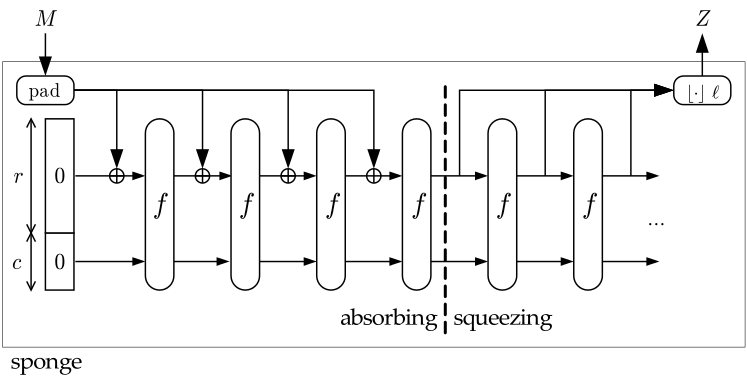
\includegraphics[width=0.5\textwidth]{images/Sponge-150.png}
  \caption{The sponge construction.}
  \label{fig:sponge}
\end{figure}

\noindent A sponge function is made up of three components: a state memory $S$ containing $b$ bits, a function $f: \left\{0,1\right\}^b \rightarrow \left\{0,1\right\}^b$ and a padding function $P$.  \cite{keccak_team,sponge_function_2023}

\begin{itemize}
  \item $S$ is divided into two parts: the rate $r$ and the capacity $c$. The rate is the part of the state that is XORed with the input message, while the capacity is the part that is not. The capacity is also the part that is permuted by the function $f$
  \item $f$ produces a pseudo random permutation of the $2^b$ possible states
  \item $P$ is a function that pads the input message to a multiple of $r$
\end{itemize}

The sponge function is performed iteratively in two phases: the \textbf{absorbing phase} and the \textbf{squeezing phase}. The padded input $M$ which is cut into $r$ bit blocks. In the absorbing phase, chucks of the input message are mixed at the beginning of the buffer using XOR operations. This can be seen in Figure \ref{fig:sponge} with the operation $r \oplus P_i$. At each step, this new buffer is again passed through $f$ causing a small amount of data to be "absorbed" into the semi-randomised buffer. \cite{keccak_team, sponge_function_2023,DBLP:journals/joc/DobraunigEMS21} \par 

In the squeezing phase, the buffer is read out in chunks of the desired output length. This is done by applying $f$ to the buffer and outputting the first $r$ bits of the result. This process is repeated until the output $Z$ with the desired length $\ell$ is reached. \cite{keccak_team,sponge_function_2023,DBLP:journals/joc/DobraunigEMS21} \par 

The last $c$ bits are neither XORed nor directly output. \par 

\subsection{The duplex construction}

\begin{figure}[htbp]
  \centering
  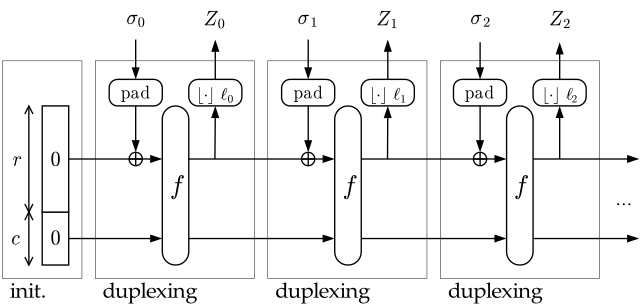
\includegraphics[width=0.5\textwidth]{images/Duplex-150.png}
  \caption{The duplex construction.}
  \label{fig:duplex}
\end{figure}

An alternation of the sponge construction is the \textbf{duplex construction}. Permutation function $f$, padding function $P$ and parameter bitrate $r$ are also used in the duplex construction, while $\sigma$ is the input string and $\ell$ is the requested number of bits. \cite{keccak_team,sponge_function_2023,guido_b_d_michaël_p_2011} \par 

While the sponge function is stateless between calls, the duplex version alternates between absorbing data into the state and squeezing data out of the state, where the output depends on all the previous inputs. \cite{guido_b_d_michaël_p_2011,cryptoeprint:2023/796} During the absorption phase, input data is XORed with the rate part of the state and then permuted using the permutation function. During the squeezing phase, output data is obtained by reading from the rate part of the state while keeping the capacity part fixed. \par

\subsection{Permutation in ASCON}
The ASCON family uses the concept of permutation in its design. The components of the encryption and hashing schemes are the two 320-bit permutations $p^a$ and $p^b$, where $a$ and $b$ are the number of times the round transformations are performed. For example, the parameters for ASCON-128 are $a = 12$ and $b = 6$, while being $a = 12$ and $b = 8$ for ASCON-128a. The permutation function is based on a substitution-permutation network (SPN) structure. \cite{DBLP:journals/joc/DobraunigEMS21, ascon_specification} \par

\subsubsection{Substitution-Permutation network}

It is a type of block cipher that uses a series of substitution and permutation operations.

\begin{figure}[htbp]
  \centering
  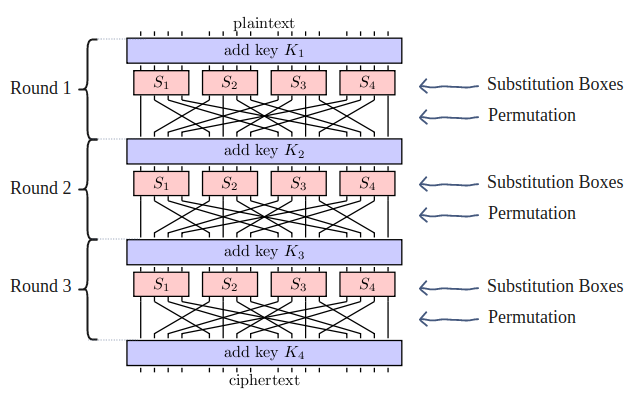
\includegraphics[width=0.5\textwidth]{images/spn.png}
  \caption{SPN structure.}
  \label{fig:spn}
\end{figure}

SPN structures consists of boxes called S-boxes that perform substitution operations and P-boxes that perform permutation operations. The S-boxes and P-boxes transform (sub-)blocks of input bits into output bits. Some common operations include simple and efficient XOR and bitwise rotation. \cite{mustafeez}

In the case of ASCON, the round transformation $p$ is based on an SPN structure. It consists of three main components: the constant addition  layer $p_C$, the substitution layer $p_S$, and the linear diffusion layer $p_L$. \cite{DBLP:journals/joc/DobraunigEMS21, ascon_specification} \par

\[p=p_C \circ p_S \circ p_L\]

In order to prepare the 320-bit state for the round transformations, the state is first divided into five 64-bit words. The round transformation $p$ is then applied to the state. \cite{DBLP:journals/joc/DobraunigEMS21} \par 

\begin{figure}[htbp]
  \centering
  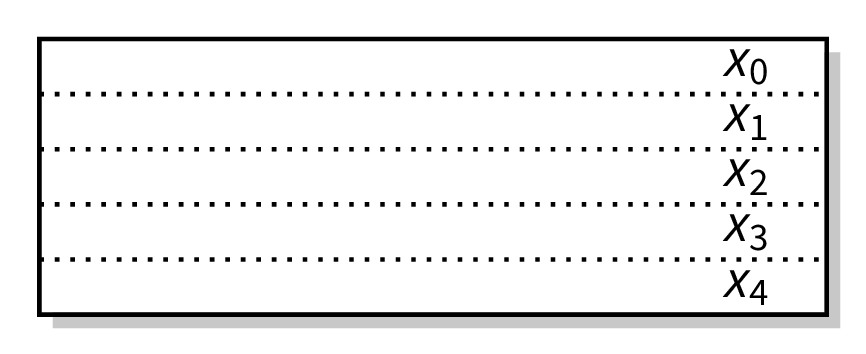
\includegraphics[width=0.5\textwidth]{images/state.png}
  \caption{The state divided into 5 64-bit words.}
  \label{fig:state}
\end{figure}

In each round of the permutation $p$ of ASCON, the following operations are performed:

\subsubsection{Constant addition layer $p_C$}
In $p_C$, a round specific 1-byte constant is XORed to $x_2$. \cite{ascon_specification, analysis_of_ascon}
  
\begin{figure}[htbp]
  \centering
  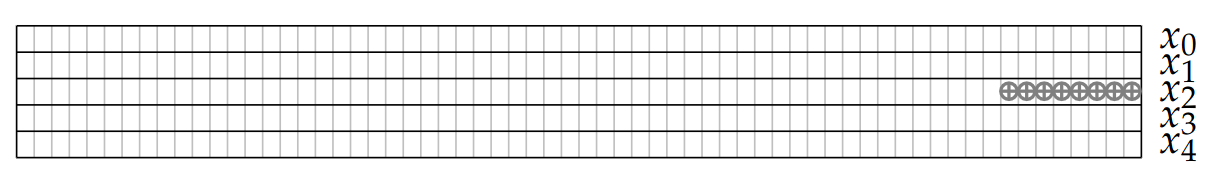
\includegraphics[width=0.8\textwidth]{images/constant.png}
  \caption{The constant addition layer $p_C$.}
  \label{fig:constant}
\end{figure}

\subsubsection{Substition layer $p_C$}
In $p_S$, a 5-bit S-box is applied to each byte of the state. It is the application of a 5-bit S-box 64 times in parallel vertically. \cite{ascon_specification, analysis_of_ascon}

\begin{figure}[htbp]
  \centering
  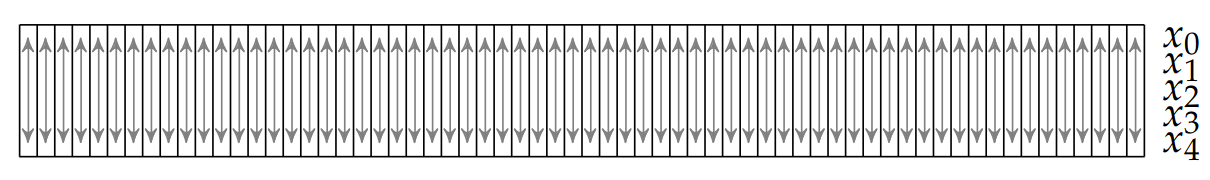
\includegraphics[width=0.8\textwidth]{images/substitution.png}
  \caption{The substitution layer $p_S$.}
  \label{fig:substition}
\end{figure}

\subsubsection{Diffusion layer $p_C$}
in $p_L$, a linear diffusion matrix is applied to the state which only consists of XOR and right rotation of the 64-bit words $x_0, x_1, x_2, x_3, x_4$. \cite{ascon_specification, analysis_of_ascon}

\begin{figure}[htbp]
  \centering
  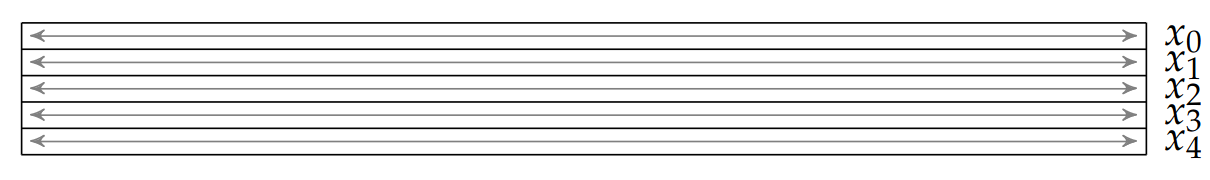
\includegraphics[width=0.8\textwidth]{images/diffusion.png}
  \caption{The diffusion layer $p_L$.}
  \label{fig:diffusion}
\end{figure}

The linear layer can be described as follows:


$\sum_0 (x_0) = x_0 \oplus (x_0 \ggg 19) \oplus (x_0 \ggg 28)$

$\sum_1 (x_1) = x_1 \oplus (x_1 \ggg 61) \oplus (x_1 \ggg 39)$

$\sum_2 (x_2) = x_2 \oplus (x_2 \ggg 1) \oplus (x_2 \ggg 6)$

$\sum_3 (x_3) = x_3 \oplus (x_3 \ggg 10) \oplus (x_3 \ggg 17)$

$\sum_4 (x_4) = x_4 \oplus (x_4 \ggg 7) \oplus (x_4 \ggg 41)$ 

\cite{ascon_specification,analysis_of_ascon}


\subsection{Design of the permutation}

There are several design criteria that need to be considered when designing a permutation for cryptographic purposes. In ASCON security was prioritised but also the performance was taken into account. \par

For the constant addition layer $p_C$, the round constants are chosen to prevent certain types of attacks and are added to the state in a simple, predictable manner for ease of computation. They are positioned strategically to facilitate efficient pipelining with other operations. \par

The S-box used in the substitution layer $p_S$ is carefully designed to meet various criteria, including invertibility, resistance against differential and linear cryptanalysis, and efficient implementation in hardware and software. \par

The linear diffusion layer mixes the bits within each word of the state. It is designed to resist linear and differential cryptanalysis while providing good diffusion. The rotation constants are chosen similar to those used in SHA-2 functions to balance performance and security. \par

\cite{DBLP:journals/joc/DobraunigEMS21}

\printbibliography

\end{document}
